\documentclass[10pt, a4paper]{article}
\usepackage[utf8]{inputenc}
\usepackage[brazilian]{babel}
\usepackage{lmodern}
\usepackage[left=2cm, right=2cm, top=2cm, bottom=2.5cm]{geometry}
\usepackage{indentfirst}
\usepackage[inline]{enumitem}

\usepackage[pensi]{zeus}

\title{Estudo em Grupo}
\author{Guilherme Zeus Moura}
\mail{zeusdanmou@gmail.com}
\titlel{Turma Olímpica}
\titler{{\footnotesize v. 1} -- 15 de Abril de 2020}

\renewcommand{\playerA}[1]{Guilherme}
\renewcommand{\playerB}[1]{Zeus}

\begin{document}	
	\zeustitle

	\problem{math/hmmt/2020/A/4}
	\problem{math/imosl/2009/C1}
	\begin{prob}[Berkeley Math Circle 2000]
		$n$ squares in an infinite grid are coloured black; the rest are coloured white. When a square is the opposite colour from $2$ or more of its $4$ neighbours, its colour may be switched. Eventually, we get to having $2017$ black squares, no two of which border along an edge, and all other squares white. Prove that $n \ge 2017$.
	\end{prob}
	\begin{prob}
		A maze consists of a finite grid of squares where the boundary and some internal
edges are “walls” that cannot be crossed. For example:

	\begin{center}
		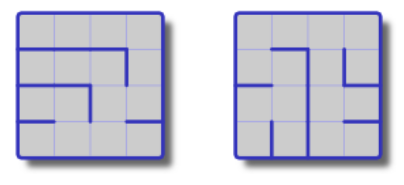
\includegraphics[width=0.4\textwidth]{pic.png}
	\end{center}
	Two mazes are given, each with a robot in the top-left square. You may give a list of directions (up, down, left, or right) to the robots. Both robots will independently follow the same list of directions. For each direction, the robot will move one square in that direction if it can, or do nothing if there is a wall in the way. It will then proceed to the next direction, and repeat until it has gone through the whole list. Suppose that there is a list of directions that will get each robot individually from the top-left corner to the bottom-right corner of its maze. Prove there is also a list of directions that will get both robots to the bottom-right corner at the same time.

	In the example mazes above, you could give the directions ‘Right’, ‘Right’, ‘Down’, ‘Down’, ‘Down’, ‘Right’, ‘Down’, ‘Down’, ‘Left’, ‘Down’, ‘Right’.
	\end{prob}
	\begin{prob}[Colorado Math Olympiad 1997]
		On every square of a $2017 \times 2017$ board, either $(+1)$ or $(-1)$ is written. For every row, we compute the product $R_i$ of all numbers written in that row, and for every column, we compute the product $C_i$ of all numbers written in that column. Is it possible to arrange the numbers in such
a way that \[ \sum_{i=1}^{2017} (R_i + C_i) = 0? \]
	\end{prob}
\end{document}
